\section{Scale, Geometry and the Earlier Results}
\subsection{What changes from 1M to 67M}
Figure~\ref{fig:scaling} compares the new small and large experiments run in the same environment. It holds the nominal target and implementation family fixed, but does not hold every table load fixed. CQF moves from 47.68\% to 49.92\% distinct uniform load; Cuckoo's capacity rounding changes its load more substantially. The stream length, memory footprint and allocation geometry all change together. The plot therefore measures scale under the implemented sizing policies, not cache capacity in isolation.

\begin{figure}[!htbp]\centering
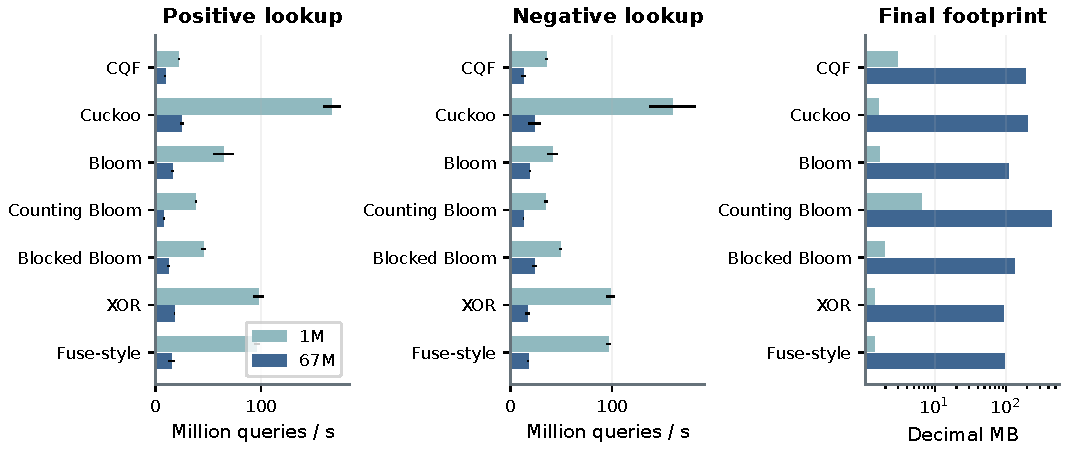
\includegraphics[width=\linewidth]{scale_comparison.pdf}
\caption{New 1M and 67M uniform query throughput and final footprint at nominal target $1/512$. Whiskers show one sample SD for throughput. Memory and capacity changes accompany the larger stream.}
\label{fig:scaling}
\end{figure}

The earlier report suggested that small filters fitting in cache could explain part of its speed ordering. The new data make that explanation more testable, but do not prove it: there are no hardware-counter measurements, controlled cache-flush experiments or native x86 runs here. Rosetta translation and fixed execution order add further reasons to keep the conclusion descriptive. The supported conclusion is that the ranking and operation costs depend on scale and configuration in this harness.

\subsection{Matched-operation-count CQF geometry sensitivity}
To separate the requested operation count from the allocation boundary, we replay 63,753,420 uniform operations against both $2^{26}$ and $2^{27}$ CQF slots, with $r=9$ and the default hash. Both configurations complete the full insert and positive-query workload in each of three repetitions. Deletion is omitted in this supplementary timing study.

\begin{table}[!htbp]\centering\small
\caption{Matched-$N$ CQF sensitivity. Rates are means $\pm$ sample SD in M/s. Holding $r=9$ while changing $q$ also changes the fingerprint width and collision estimate.}
\label{tab:geometry-control}
\begin{tabular}{@{}lrrrrr@{}}
\toprule
\textbf{Slots} & \textbf{MB} & \textbf{First FPR} & \textbf{Insert} & \textbf{Positive} & \textbf{Negative} \\
\midrule
$2^{26}$ & 93.437 & $1.85\times10^{-3}$ & 1.51 $\pm$ 0.01 & 7.63 $\pm$ 0.04 & 10.45 $\pm$ 0.07 \\
$2^{27}$ & 186.808 & $9.26\times10^{-4}$ & 1.58 $\pm$ 0.00 & 9.84 $\pm$ 0.07 & 14.25 $\pm$ 0.51 \\
\bottomrule
\end{tabular}

\end{table}

The larger table doubles final memory and reduces distinct load from 95\% to 47.5\%. It also increases $p=q+r$ from 35 to 36 bits, approximately halving the expected FPR. Any speed difference is a combined geometry effect involving run lengths, address range and fingerprint collisions. The near-full table uses \GeometrySmallBits{} bits per uniform key, close to the reference paper's 11.71; the doubled table uses \GeometryLargeBits{}. This control separates the requested operation count from the allocation boundary, while retaining the stated fingerprint-width confound.

An application must also account for the work caused by false positives. If an absent-key lookup costs $c_{\mathrm{filter}}$ in the filter and a positive answer triggers an additional cost $C$, its expected cost is $c_{\mathrm{filter}}+\hat p C$ under that lookup model. A more accurate filter can therefore be worthwhile even when its own query is slower. We do not assign a measured value to $C$ here; it is a property of the application that the microbenchmark cannot determine.
\clearpage

\subsection{Comparison with the mid-semester report and reference paper}
\begin{table}[!htbp]\centering\small
\caption{Uniform reference context for the original three filters. Insert/positive/negative rates are in M/s. Literature values are from Table~1(a) of Pandey et al.; earlier values are transcribed from the supplied report. Archived 67M values are preserved from the input ZIP; new values are measured in this session. These are separate environments, configurations and protocols, not speedup trials.}
\label{tab:history}
\begin{tabular}{@{}llrrr@{}}
\toprule
\textbf{Result source} & \textbf{Filter} & \textbf{Insert} & \textbf{Positive} & \textbf{Negative} \\
\midrule
Reference paper & CQF & 11.19 & 11.16 & 25.93 \\
Reference paper & Cuckoo & 14.25 & 18.87 & 18.84 \\
Reference paper & Bloom & 2.84 & 2.55 & 11.56 \\
Mid-semester & CQF & 8.33 & 17.06 & 23.91 \\
Mid-semester & Cuckoo & 22.75 & 125.47 & 128.23 \\
Mid-semester & Bloom & 30.22 & 30.16 & 31.04 \\
Archived 67M & CQF & 3.85 & 7.03 & 9.92 \\
Archived 67M & Cuckoo & 18.15 & 19.22 & 18.76 \\
Archived 67M & Bloom & 6.61 & 7.44 & 12.30 \\
New 67M & CQF & 1.47 & 9.23 & 12.80 \\
New 67M & Cuckoo & 21.43 & 25.14 & 23.93 \\
New 67M & Bloom & 11.88 & 16.20 & 19.25 \\
\bottomrule
\end{tabular}

\end{table}

The mid-semester baseline used 996,148 operations and a CQF near 95\% load. Its values are retained exactly as reported, even where the supplied archive also contains later validation numbers. The supplied archive's 67M study extends the original three filters and supplies an earlier hash study; it does not contain an all-seven 67M measurement. Our new large experiment supplies that missing comparison.

The reference paper uses an Intel Skylake machine and samples performance through successive load levels. It excludes input generation, as we do, but its implementation versions and hardware differ. Its skewed-data result also identifies the ordinary Cuckoo filter's duplicate limitation, while our exact stopping point is determined by our stream. The meaningful agreements are completion behaviour and the roles of counting, space and load; the absolute rates are contextual reference values~\cite{pandey2017}.

The paper's CQF-over-Counting-Bloom speed ordering is not reproduced uniformly in our new results. Our Counting Bloom reaches \CountingBloomInsertSkewLarge{}\Mops{} on skewed insertion, compared with \CqfInsertSkewLarge{}\Mops{} for CQF. CQF leads in positive-query throughput, while Counting Bloom leads in negative-query throughput. The packed-counter overflow implementation, distinct-aware sizing and translated host all differ from the published setup. These measurements describe the configured implementations in this study and leave native, matched-configuration replication as follow-up work.

The public repository ends at commit \texttt{fe184baa6933} (9 November 2026), which adds hash and paper-scale studies~\cite{projectcode}. The supplied Phase-3 ZIP adds the four new filters and is our experimental source snapshot. The public API returned no pull-request entries; this provenance is a verified source history, not a PR timeline.

\subsection{What can be carried across these comparisons}
Three kinds of agreement should be distinguished. \textit{Semantic agreement} asks whether the implementation performs the required task: CQF and Counting Bloom retain repeated occurrences, while this Cuckoo configuration runs out of room for copies. \textit{Configuration agreement} asks whether the same capacity, fingerprint width and cardinality knowledge were used. \textit{Numerical agreement} asks whether rates match after hardware, software and timing conventions are controlled. This study establishes the first, records the second, and gives contextual rather than replicated evidence for the third.

The distinction matters even at small scale. Moving from 996,148 to exactly 1M operations adds only about 0.39\% more input, yet crosses the CQF allocation boundary and doubles its slot count. The archived and new 67M Zipf generators also realize slightly different distinct sets: 229,118 versus 229,115 keys. The difference is small, but it illustrates why the report keeps separate input audits instead of treating a shared seed as proof of identical data. Our extension adds a common seven-family record and controls that make these operating points visible; it does not convert cross-environment rates into algorithmic speedups.
\clearpage

\subsection{Sensitivity to the nominal error target}
We also replay the 67M streams at nominal targets $1/256$ and $1/1024$. These two supplementary configurations have one timing pass each; only the main $1/512$ configuration has three. The sweep checks parameterization and space/accuracy trends. It does not provide repeated performance evidence at every error target.

\begin{figure}[!htbp]\centering
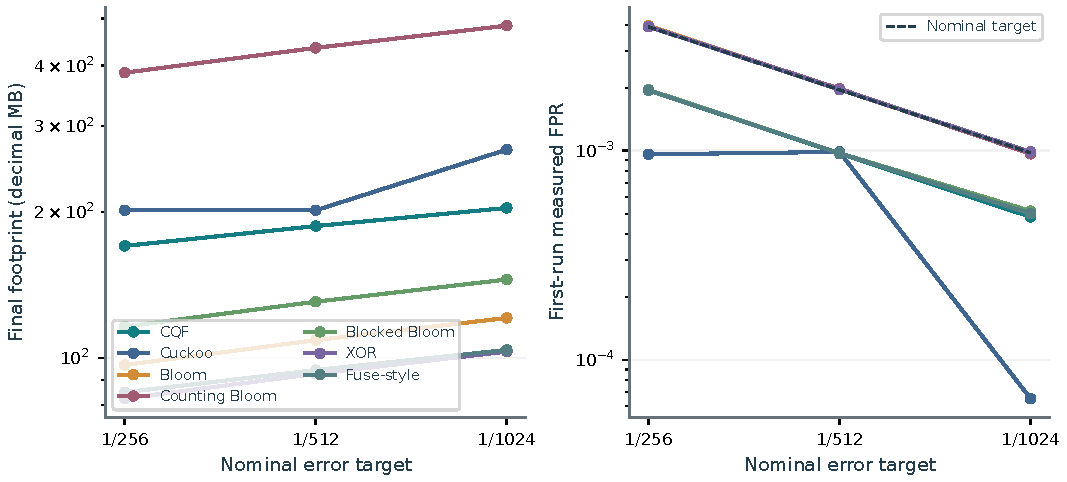
\includegraphics[width=\linewidth]{fpr_sensitivity.pdf}
\caption{67M uniform space and measured FPR across three nominal targets. Each point uses the first pass; the end targets are single-pass supplementary experiments. Fuse-style retains one guard bit beyond XOR. Changes in achieved accuracy and footprint should be read together.}
\label{fig:sensitivity}
\end{figure}

\begin{table}[!htbp]\centering\small
\caption{Uniform target sweep at 67M operations. Column labels 256, 512 and 1024 denote nominal targets $1/256$, $1/512$ and $1/1024$. Memory is decimal MB; first-pass FPRs are in units of $10^{-3}$. The end targets have one timing pass, so this table describes space and sampled accuracy, not repeated speed rankings.}
\label{tab:target-sweep}
\begin{tabular}{@{}lrrrrrr@{}}
\toprule
\textbf{Filter} & \textbf{MB: 256} & \textbf{MB: 512} & \textbf{MB: 1024} & \textbf{FPR: 256} & \textbf{FPR: 512} & \textbf{FPR: 1024} \\
\midrule
CQF & 170.02 & 186.81 & 203.60 & 1.9408 & 0.9692 & 0.4827 \\
Cuckoo & 201.33 & 201.33 & 268.44 & 0.9607 & 0.9865 & 0.0653 \\
Bloom & 96.66 & 108.74 & 120.83 & 3.9591 & 1.9616 & 0.9826 \\
Counting Bloom & 386.64 & 434.97 & 483.30 & 3.9207 & 1.9771 & 0.9662 \\
Blocked Bloom & 115.99 & 130.49 & 144.99 & 1.9535 & 0.9730 & 0.5149 \\
XOR & 82.41 & 92.71 & 103.01 & 3.9159 & 1.9597 & 0.9866 \\
Fuse-style & 84.93 & 94.37 & 103.81 & 1.9409 & 0.9725 & 0.5003 \\
\bottomrule
\end{tabular}

\end{table}

The CQF keeps $q=27$ throughout the sweep and increases $r$ from 8 to 10. Each additional remainder bit adds about 16.79\,MB to the primary allocation and approximately halves the collision estimate. Bloom-family storage also grows as the target tightens, with the number of probes rising from 8 to 10. Counting Bloom pays four bits per base cell before overflow, so the same sizing change carries a larger absolute space cost.

Cuckoo exposes a different parameter effect. Its supported fingerprint widths keep it at 12 bits for the first two targets, then move it to 16 bits for $1/1024$. Memory jumps from 201.33 to 268.44\,MB, while the measured FPR falls well below the requested target. A smooth nominal-target axis therefore need not produce a smooth space curve. The guard choices in Blocked Bloom and Fuse-style likewise leave them below the common target. Equalizing the target input is useful for checking the harness; comparing equal achieved accuracy would require selecting different configurations.
\finding{Accuracy is purchased in implementation-specific increments. The relevant comparison is the achieved error rate together with its storage and operation cost, not the target label alone.}
\clearpage
